% Generated by plot_retention_scores.py; edit the generator instead.
\section{Retention--Score Curves}
\label{app:retention-curves}

This appendix plots all 60 matched configurations and their benchmark and task-family summaries. The seven benchmark summaries reproduce the aggregate rows in Tables~\ref{tab:results-graphkv}--\ref{tab:results-kvzip}. Each aggregate is the arithmetic mean of its unrounded configuration scores, independently at each retention ratio. All plots use absolute native-evaluator scores (0--100) and the same method colors. Each panel has a zoomed linear y-axis enclosing all three methods and their full-cache baselines. Y-axis ranges vary across panels; tick labels show the actual scores. Flat and near-flat panels span at least two score points, and identical constant curves are explicitly marked.

Solid curves show the three methods at 20, 30, 40, 50, 75, and 100\% retention. 17 of 98 panels additionally include 5 and 10\% retention: the 11 SCBench base tasks, their aggregate mean, and their four family panels. These two extra points were evaluated only for the 11 SCBench base tasks; the 16 length variants and all RULER configurations are unaffected and still span 20--100\%. Dashed horizontal lines show each method's own measured full-cache score, using the matching color; one gray dashed line is used when all three full-cache scores coincide. Coincident curves and nearly equal baselines may overlap. The full-cache point is included at 100\% retention. SCBench base-task and all-variant means are distinguished; RULER 64K contains only seven selected tasks.

SCBench families follow Section~3.1 and Table~2 of \citet{li2025scbench}: string retrieval, semantic retrieval, global information processing, and multi-tasking. Chinese QA is absent from our semantic-retrieval subset. Prepared length variants inherit their base task's family. RULER families and needle-retrieval subtypes follow Section~3 of \citet{hsieh2024ruler}. One-task families repeat their individual curve for convenient comparison. The deployed combined scores for mixed SCBench and Many-shot tasks are retained; component scores are not separately available in the table snapshot. Unevaluated configurations have no curves.

\paragraph{Plot guide.}
Benchmark summaries (Figures~\ref{fig:retention-suite-overview}--\ref{fig:retention-ruler-lengths}); SCBench task families (Figures~\ref{fig:retention-scbench-families-base-tasks}--\ref{fig:retention-scbench-families-all-variants}); RULER task families (Figures~\ref{fig:retention-ruler-4k}--\ref{fig:retention-ruler-64k}); RULER retrieval subtypes (Figures~\ref{fig:retention-ruler-retrieval-subtypes-4k}--\ref{fig:retention-ruler-retrieval-subtypes-64k}); SCBench individual tasks (Figures~\ref{fig:retention-scbench-tasks-1}--\ref{fig:retention-scbench-tasks-5}); RULER 4K individual tasks (Figures~\ref{fig:retention-ruler-4k-tasks-1}--\ref{fig:retention-ruler-4k-tasks-3}); RULER 8K individual tasks (Figures~\ref{fig:retention-ruler-8k-tasks-1}--\ref{fig:retention-ruler-8k-tasks-3}); RULER 64K individual tasks (Figures~\ref{fig:retention-ruler-64k-tasks-1}--\ref{fig:retention-ruler-64k-tasks-2}).
\clearpage

\subsection{Benchmark summaries}

\begin{figure}[!ht]
\centering
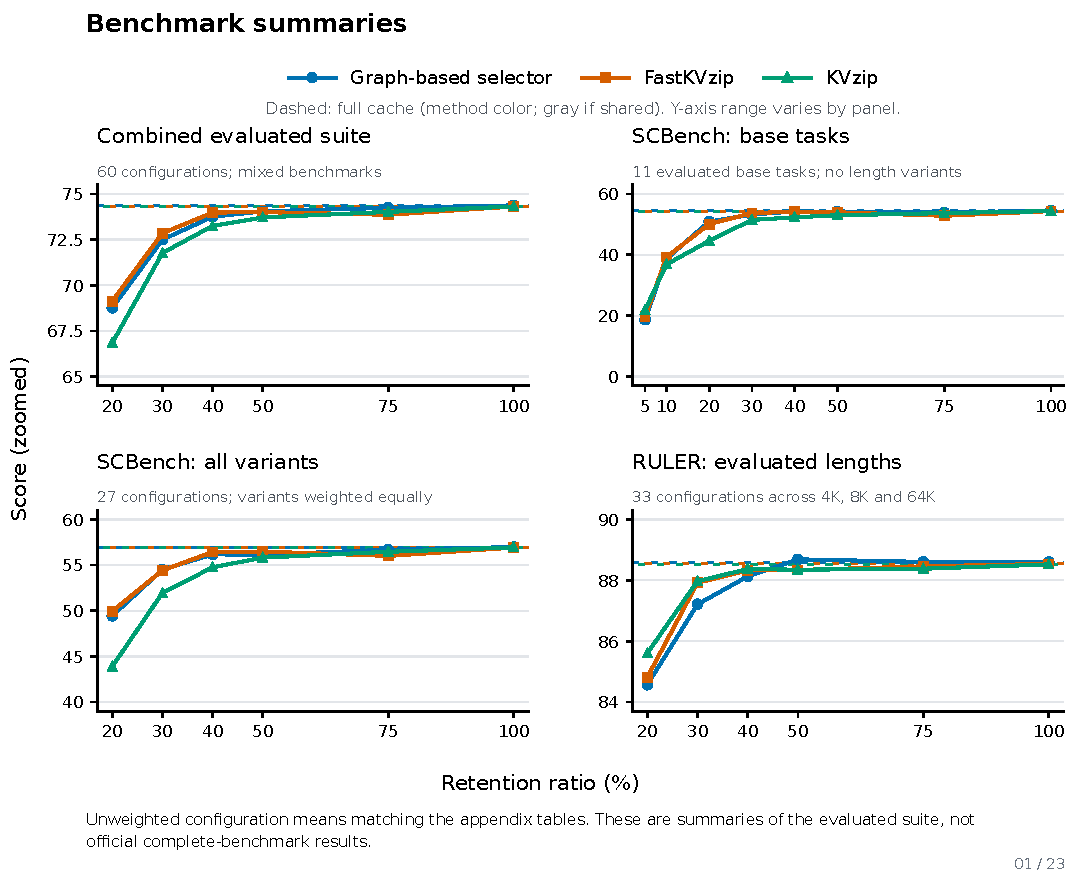
\includegraphics[width=\linewidth]{figures/retention-curves/01-suite-overview.pdf}
\caption{Benchmark summaries.}
\label{fig:retention-suite-overview}
\end{figure}
\clearpage

\begin{figure}[!ht]
\centering
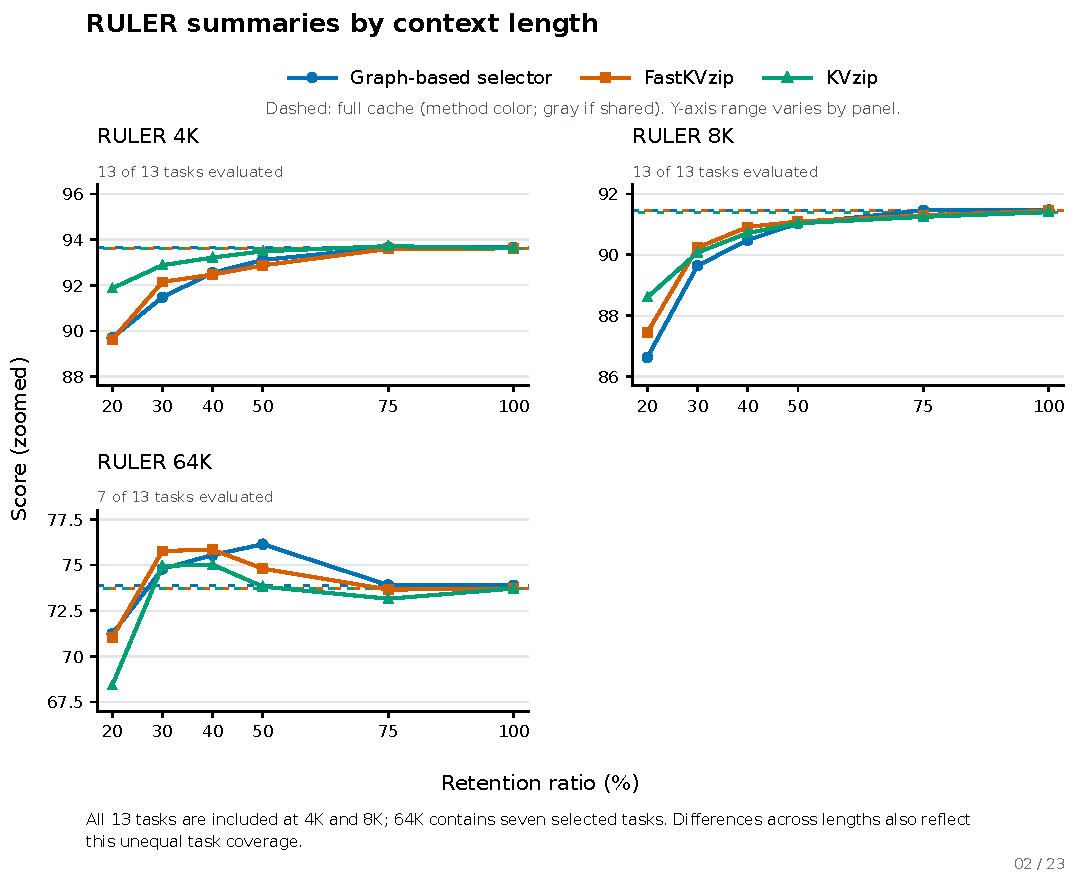
\includegraphics[width=\linewidth]{figures/retention-curves/02-ruler-lengths.pdf}
\caption{RULER summaries by context length.}
\label{fig:retention-ruler-lengths}
\end{figure}
\clearpage

\subsection{SCBench task families}

\begin{figure}[!ht]
\centering
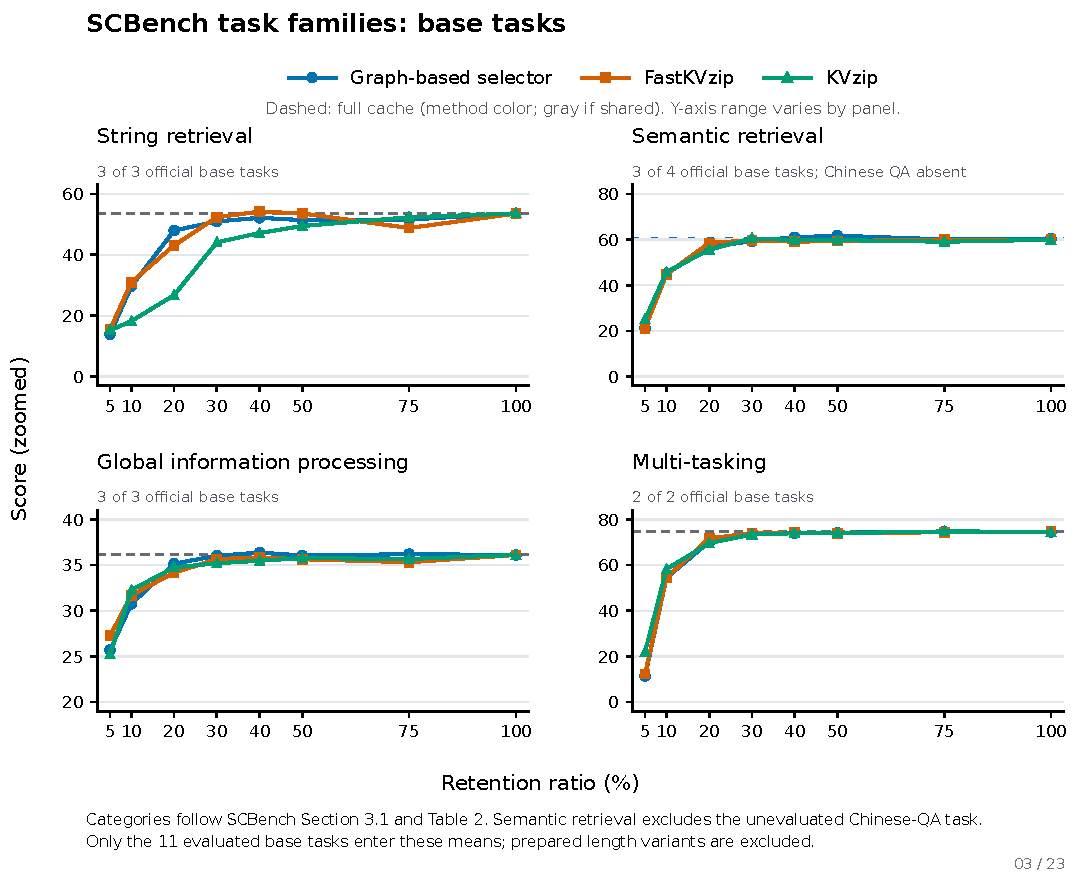
\includegraphics[width=\linewidth]{figures/retention-curves/03-scbench-families-base-tasks.pdf}
\caption{SCBench task families: base tasks.}
\label{fig:retention-scbench-families-base-tasks}
\end{figure}
\clearpage

\begin{figure}[!ht]
\centering
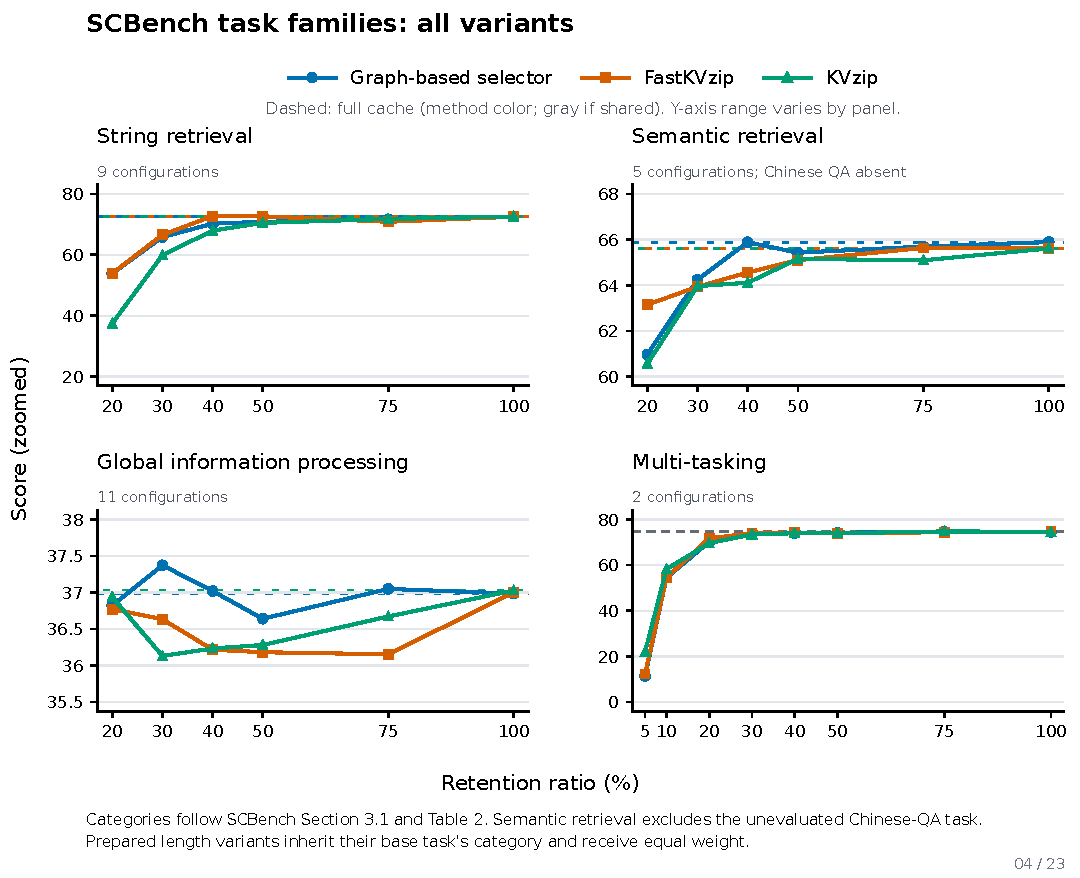
\includegraphics[width=\linewidth]{figures/retention-curves/04-scbench-families-all-variants.pdf}
\caption{SCBench task families: all variants.}
\label{fig:retention-scbench-families-all-variants}
\end{figure}
\clearpage

\subsection{RULER task families}

\begin{figure}[!ht]
\centering
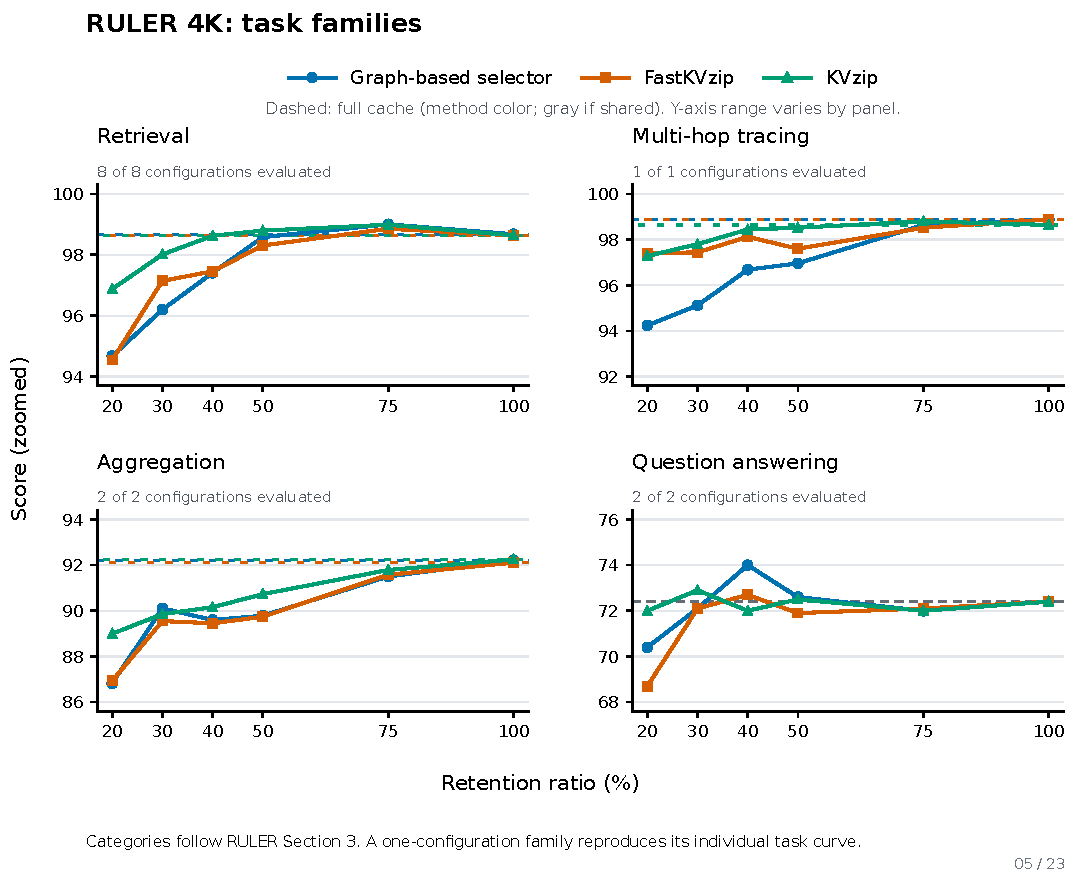
\includegraphics[width=\linewidth]{figures/retention-curves/05-ruler-4k.pdf}
\caption{RULER 4K: task families.}
\label{fig:retention-ruler-4k}
\end{figure}
\clearpage

\begin{figure}[!ht]
\centering
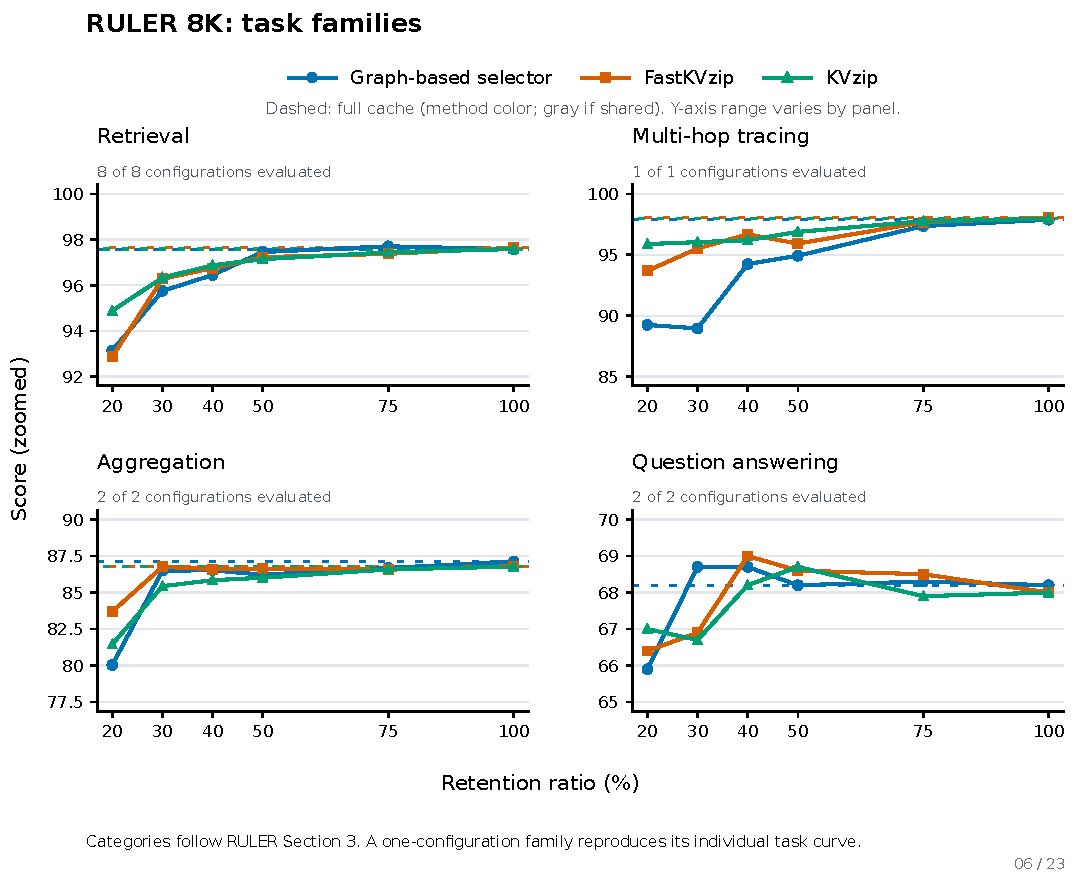
\includegraphics[width=\linewidth]{figures/retention-curves/06-ruler-8k.pdf}
\caption{RULER 8K: task families.}
\label{fig:retention-ruler-8k}
\end{figure}
\clearpage

\begin{figure}[!ht]
\centering
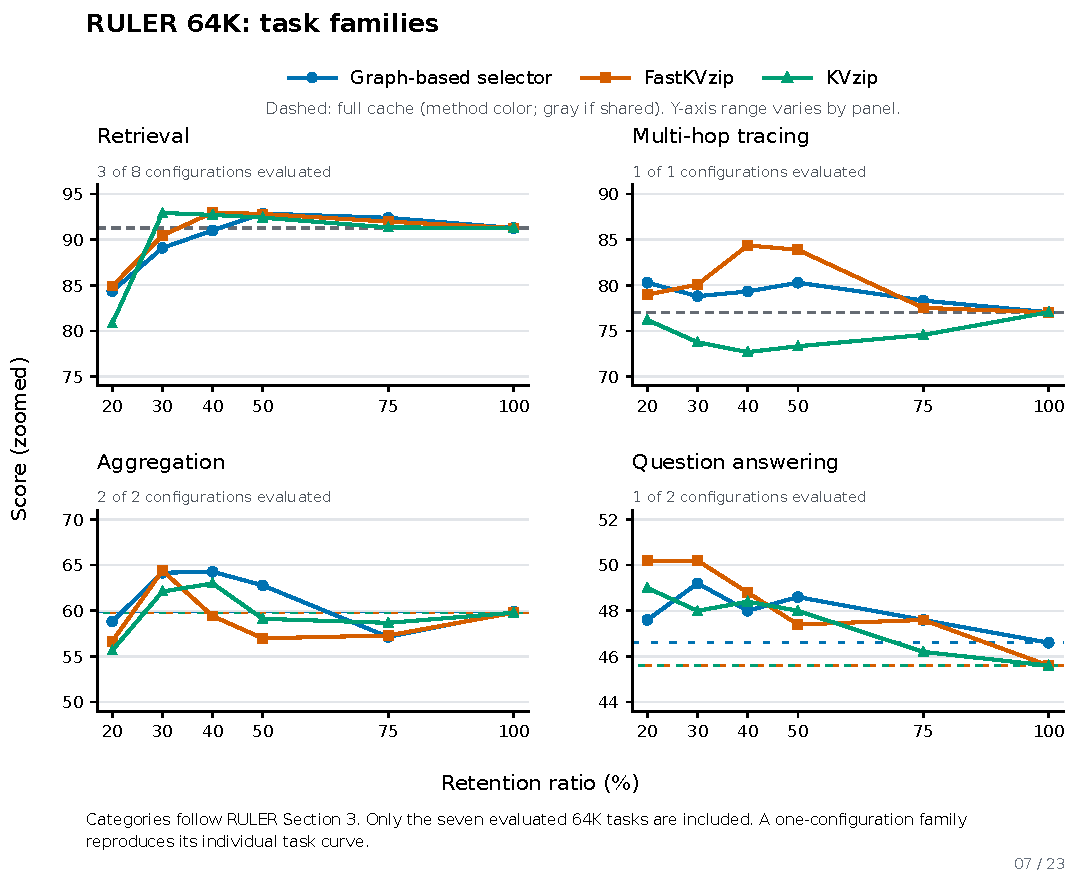
\includegraphics[width=\linewidth]{figures/retention-curves/07-ruler-64k.pdf}
\caption{RULER 64K: task families.}
\label{fig:retention-ruler-64k}
\end{figure}
\clearpage

\subsection{RULER retrieval subtypes}

\begin{figure}[!ht]
\centering
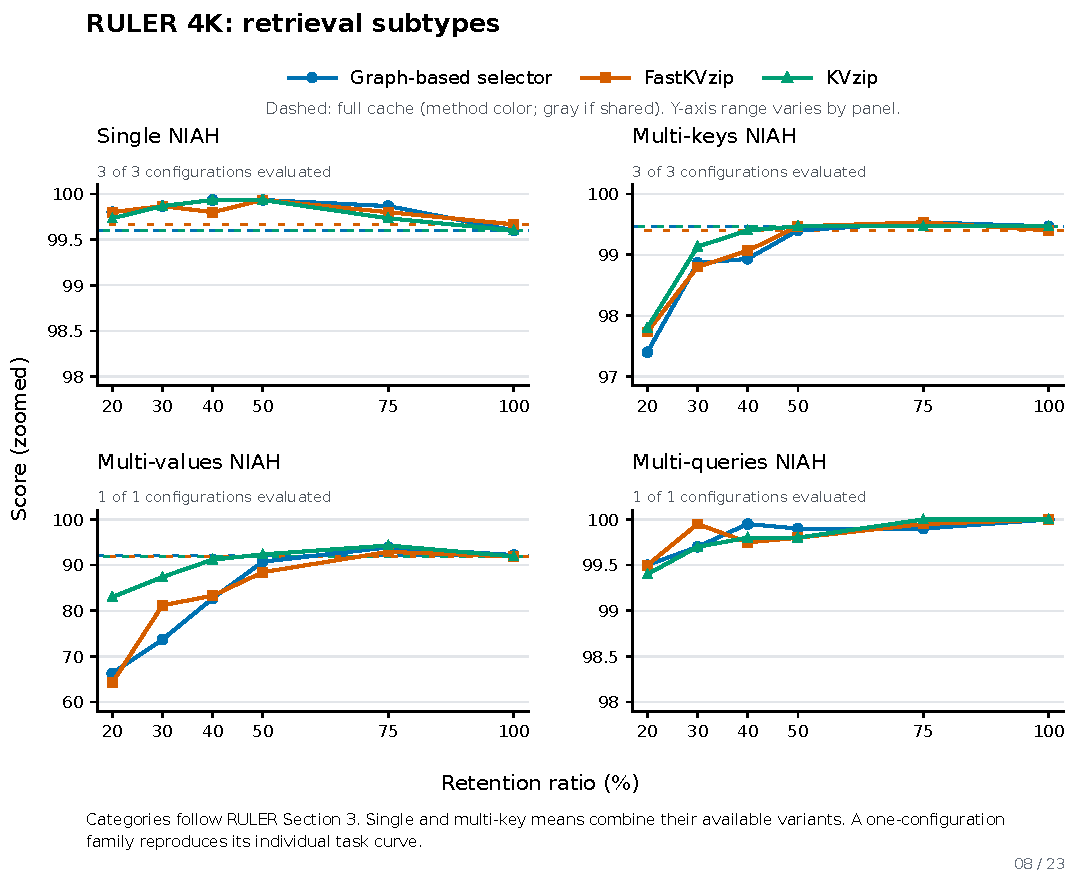
\includegraphics[width=\linewidth]{figures/retention-curves/08-ruler-retrieval-subtypes-4k.pdf}
\caption{RULER 4K: retrieval subtypes.}
\label{fig:retention-ruler-retrieval-subtypes-4k}
\end{figure}
\clearpage

\begin{figure}[!ht]
\centering
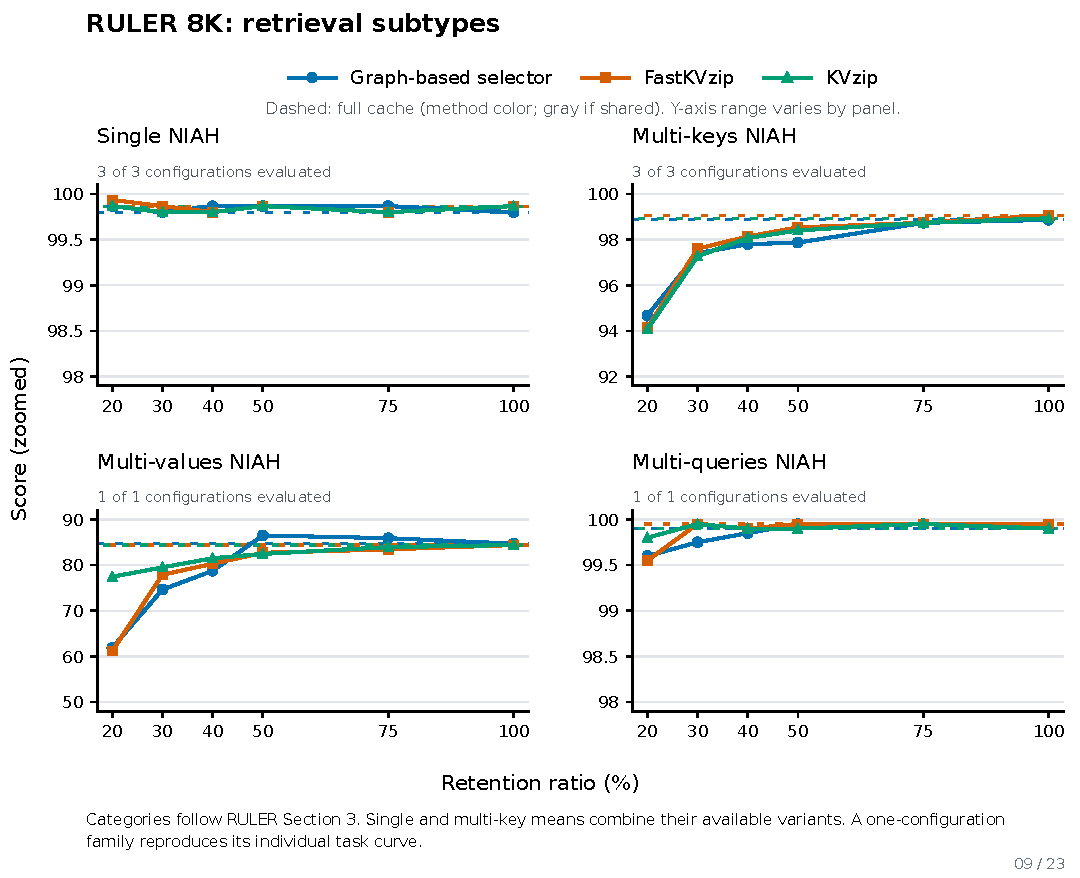
\includegraphics[width=\linewidth]{figures/retention-curves/09-ruler-retrieval-subtypes-8k.pdf}
\caption{RULER 8K: retrieval subtypes.}
\label{fig:retention-ruler-retrieval-subtypes-8k}
\end{figure}
\clearpage

\begin{figure}[!ht]
\centering
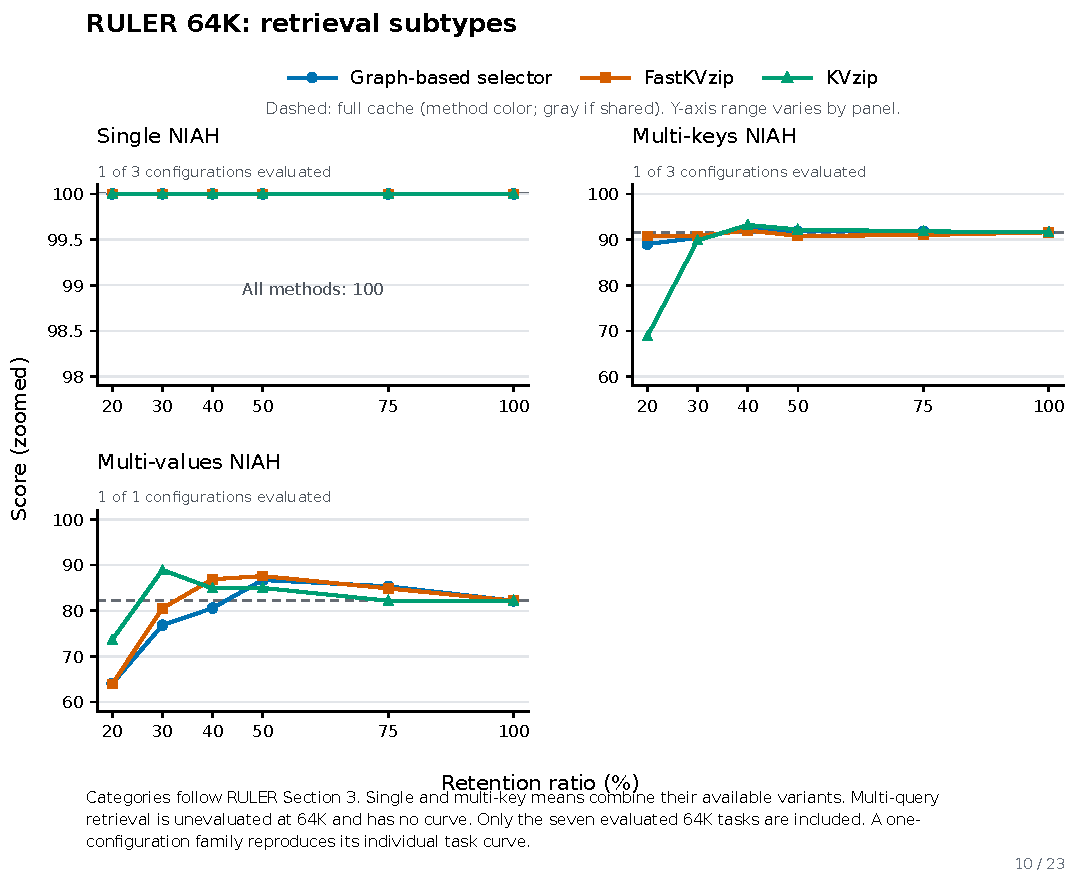
\includegraphics[width=\linewidth]{figures/retention-curves/10-ruler-retrieval-subtypes-64k.pdf}
\caption{RULER 64K: retrieval subtypes.}
\label{fig:retention-ruler-retrieval-subtypes-64k}
\end{figure}
\clearpage

\subsection{SCBench individual tasks}

\begin{figure}[!ht]
\centering
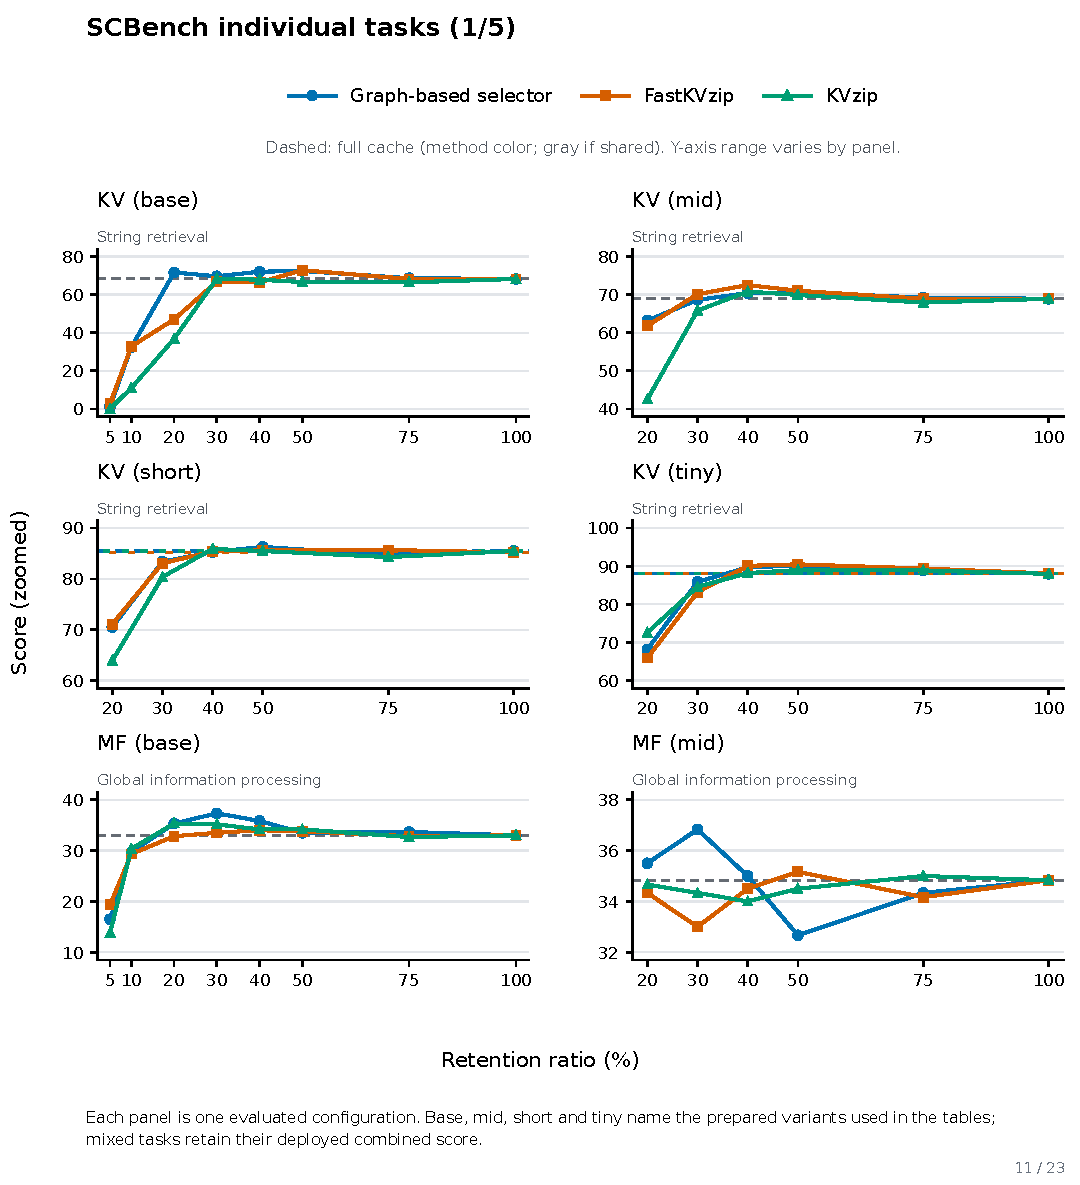
\includegraphics[width=\linewidth]{figures/retention-curves/11-scbench-tasks-1.pdf}
\caption{SCBench individual tasks (1/5).}
\label{fig:retention-scbench-tasks-1}
\end{figure}
\clearpage

\begin{figure}[!ht]
\centering
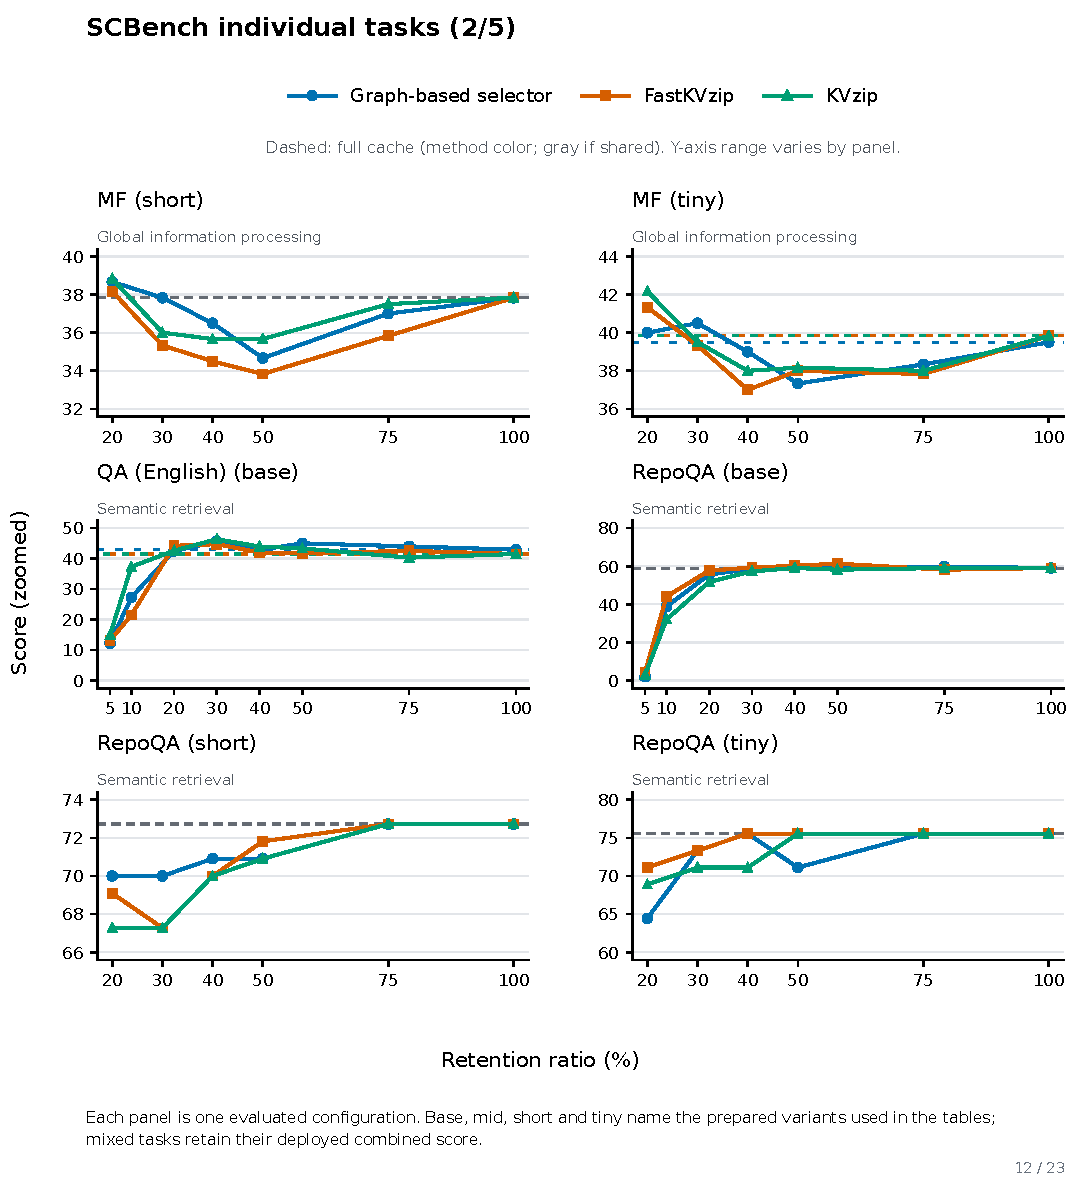
\includegraphics[width=\linewidth]{figures/retention-curves/12-scbench-tasks-2.pdf}
\caption{SCBench individual tasks (2/5).}
\label{fig:retention-scbench-tasks-2}
\end{figure}
\clearpage

\begin{figure}[!ht]
\centering
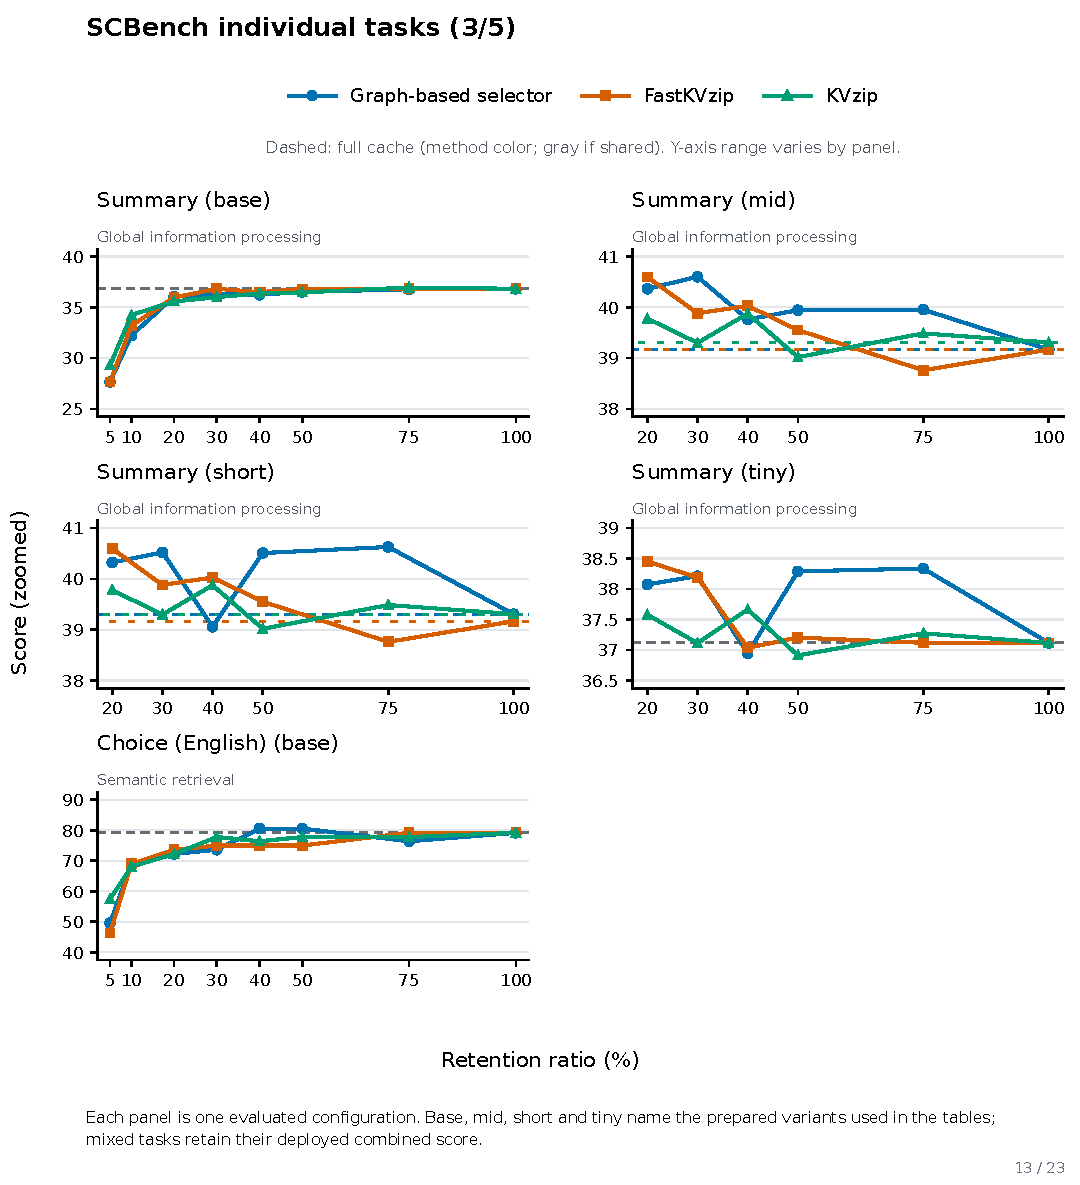
\includegraphics[width=\linewidth]{figures/retention-curves/13-scbench-tasks-3.pdf}
\caption{SCBench individual tasks (3/5).}
\label{fig:retention-scbench-tasks-3}
\end{figure}
\clearpage

\begin{figure}[!ht]
\centering
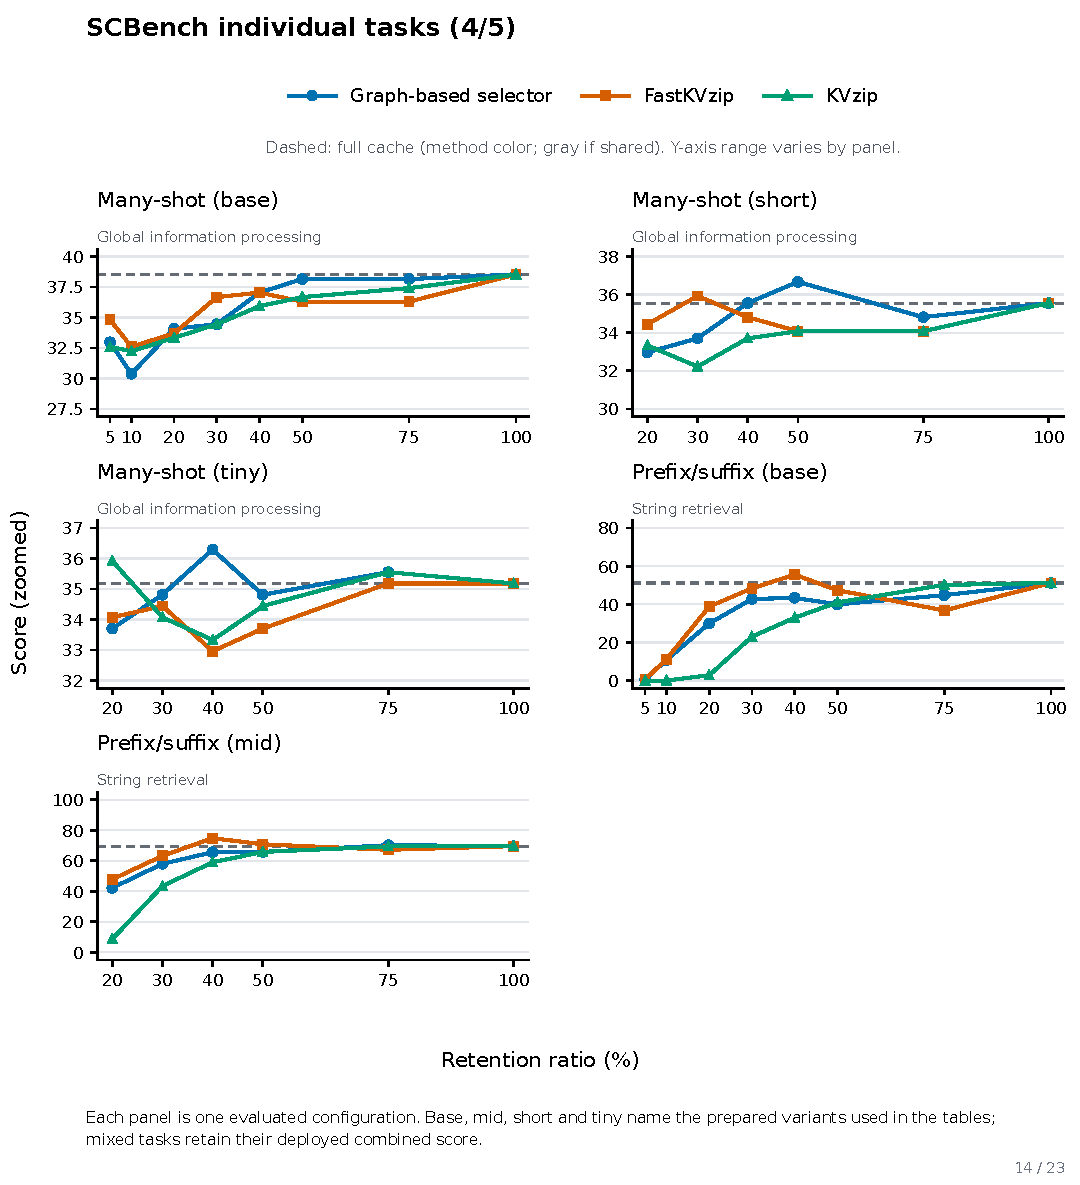
\includegraphics[width=\linewidth]{figures/retention-curves/14-scbench-tasks-4.pdf}
\caption{SCBench individual tasks (4/5).}
\label{fig:retention-scbench-tasks-4}
\end{figure}
\clearpage

\begin{figure}[!ht]
\centering
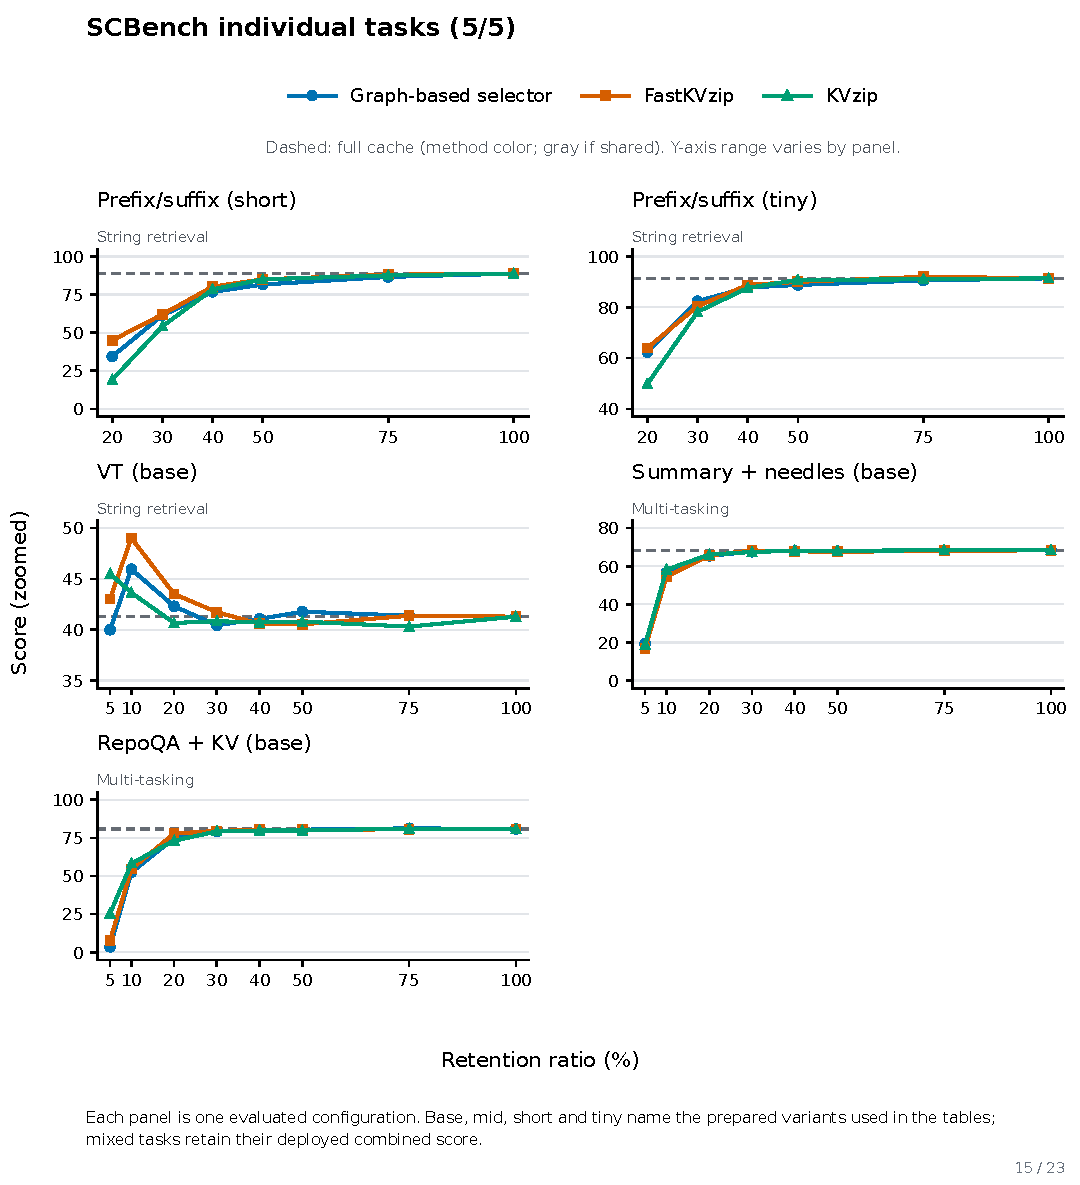
\includegraphics[width=\linewidth]{figures/retention-curves/15-scbench-tasks-5.pdf}
\caption{SCBench individual tasks (5/5).}
\label{fig:retention-scbench-tasks-5}
\end{figure}
\clearpage

\subsection{RULER 4K individual tasks}

\begin{figure}[!ht]
\centering
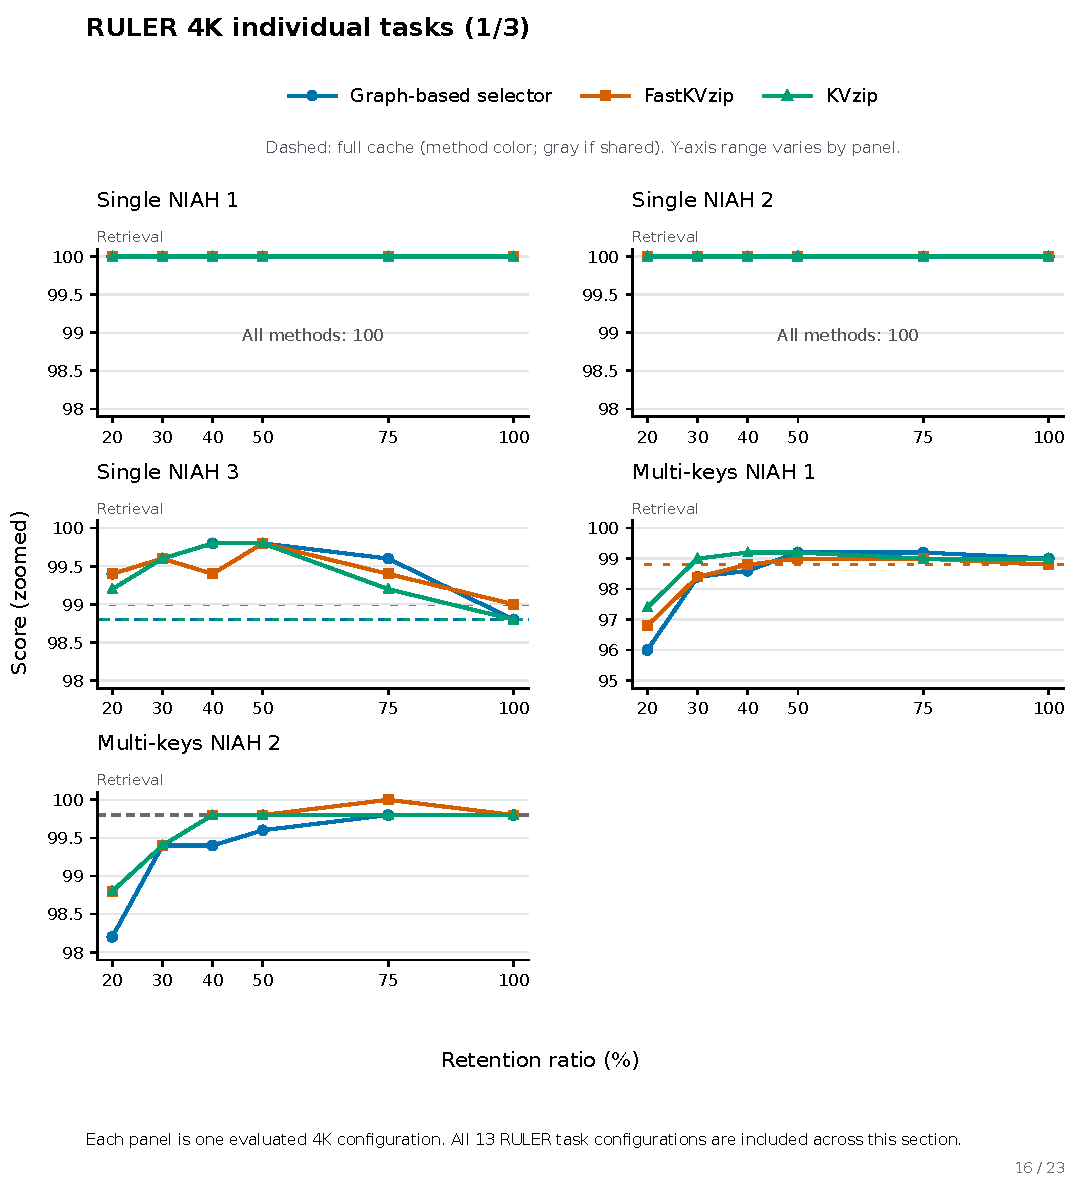
\includegraphics[width=\linewidth]{figures/retention-curves/16-ruler-4k-tasks-1.pdf}
\caption{RULER 4K individual tasks (1/3).}
\label{fig:retention-ruler-4k-tasks-1}
\end{figure}
\clearpage

\begin{figure}[!ht]
\centering
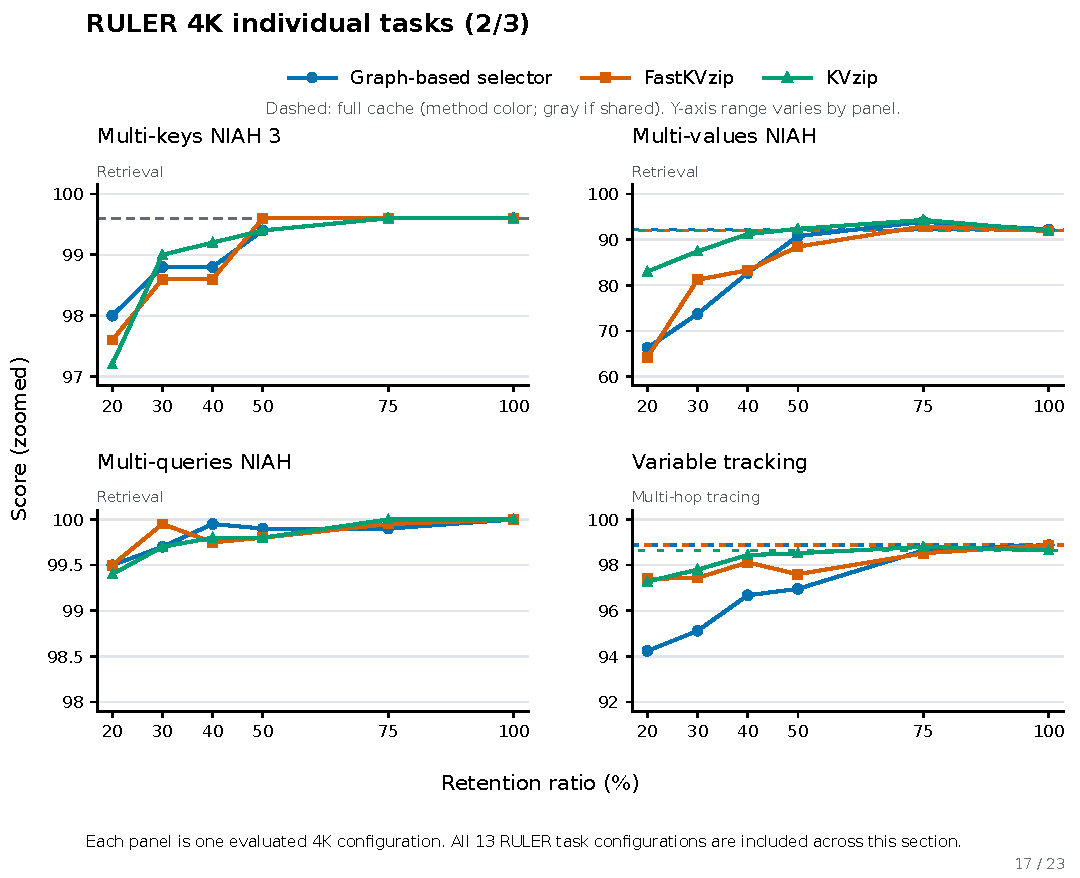
\includegraphics[width=\linewidth]{figures/retention-curves/17-ruler-4k-tasks-2.pdf}
\caption{RULER 4K individual tasks (2/3).}
\label{fig:retention-ruler-4k-tasks-2}
\end{figure}
\clearpage

\begin{figure}[!ht]
\centering
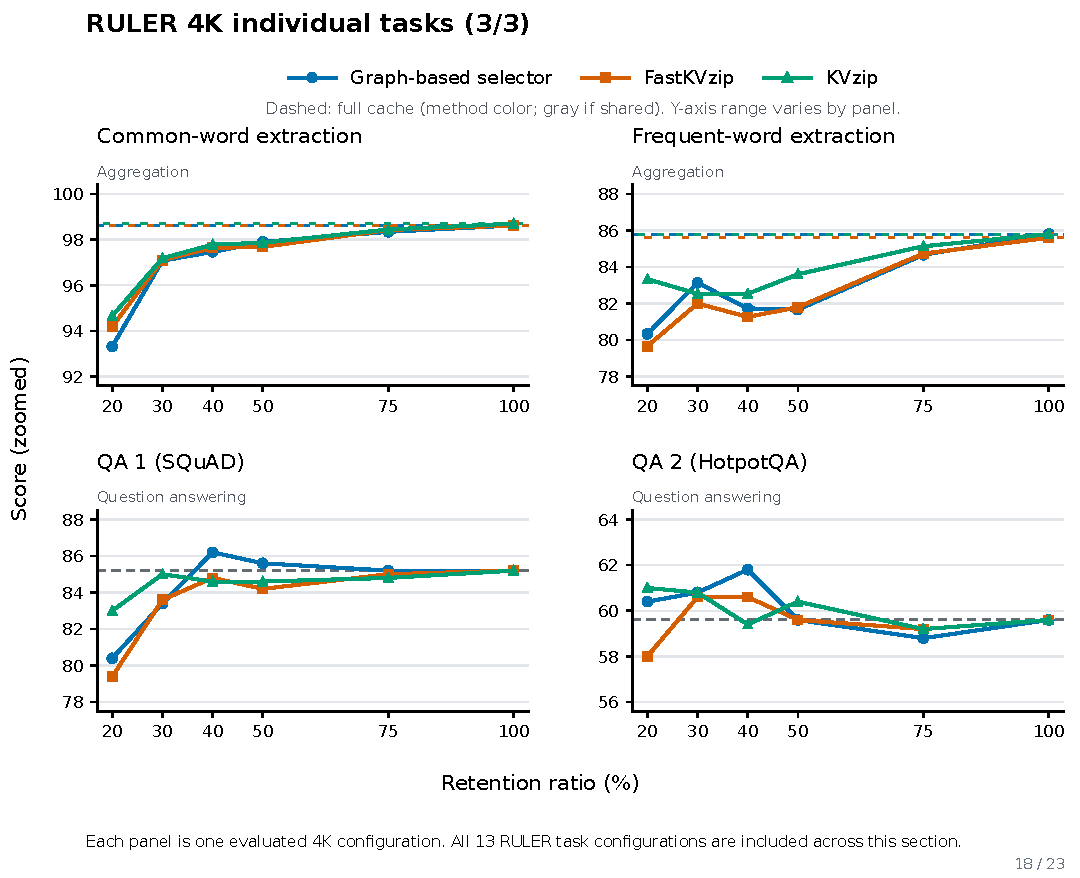
\includegraphics[width=\linewidth]{figures/retention-curves/18-ruler-4k-tasks-3.pdf}
\caption{RULER 4K individual tasks (3/3).}
\label{fig:retention-ruler-4k-tasks-3}
\end{figure}
\clearpage

\subsection{RULER 8K individual tasks}

\begin{figure}[!ht]
\centering
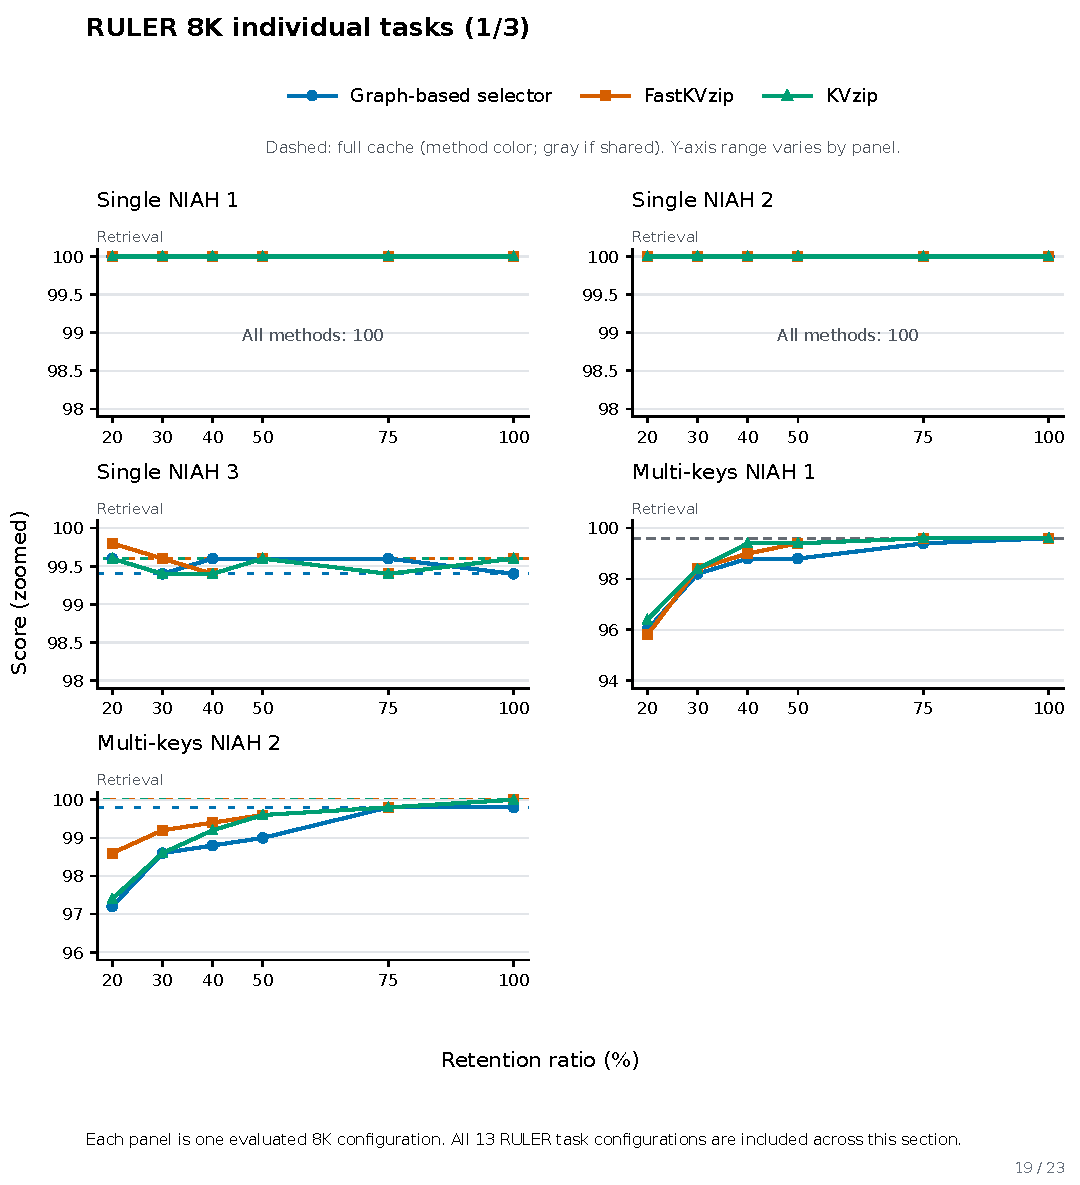
\includegraphics[width=\linewidth]{figures/retention-curves/19-ruler-8k-tasks-1.pdf}
\caption{RULER 8K individual tasks (1/3).}
\label{fig:retention-ruler-8k-tasks-1}
\end{figure}
\clearpage

\begin{figure}[!ht]
\centering
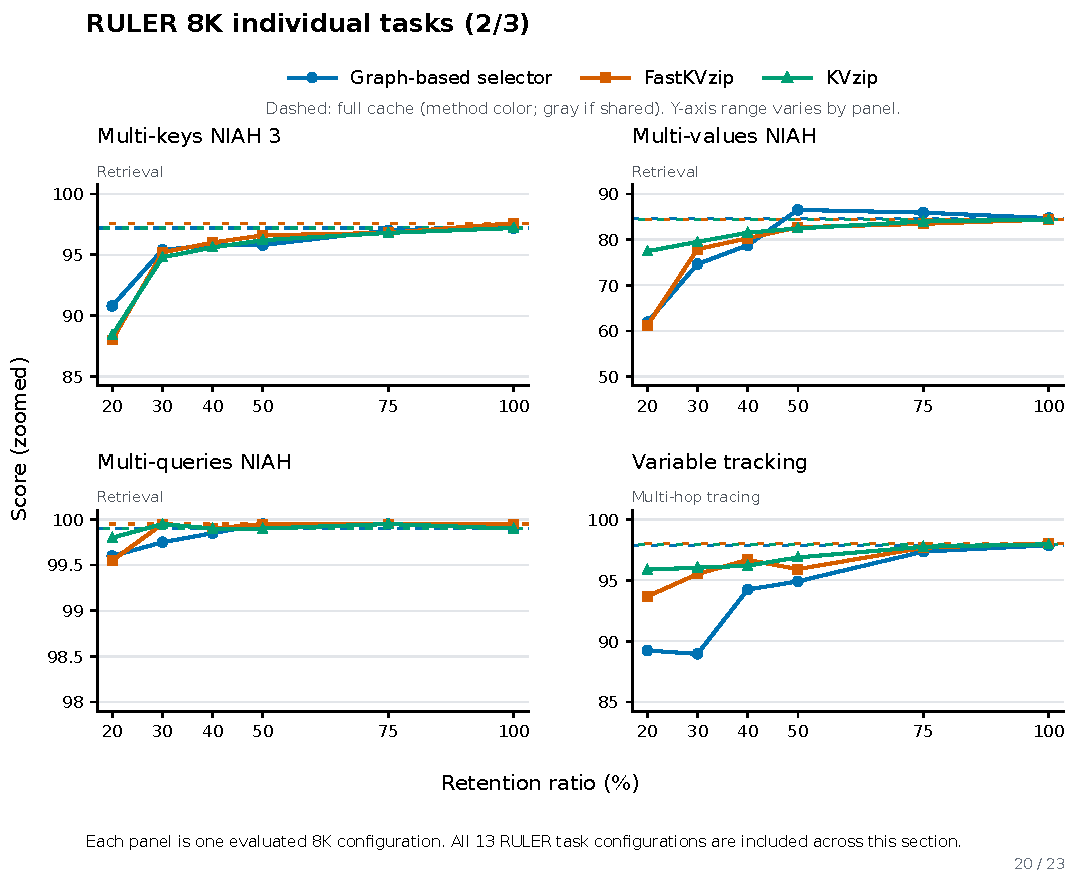
\includegraphics[width=\linewidth]{figures/retention-curves/20-ruler-8k-tasks-2.pdf}
\caption{RULER 8K individual tasks (2/3).}
\label{fig:retention-ruler-8k-tasks-2}
\end{figure}
\clearpage

\begin{figure}[!ht]
\centering
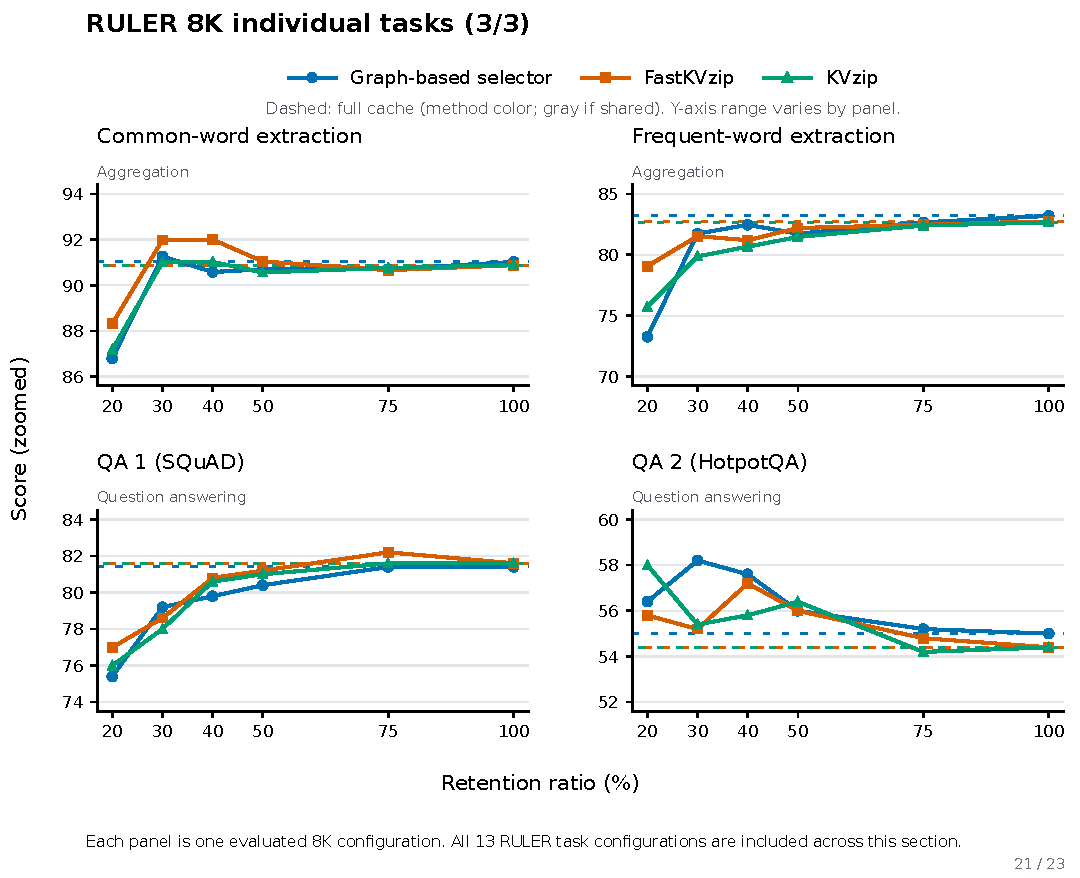
\includegraphics[width=\linewidth]{figures/retention-curves/21-ruler-8k-tasks-3.pdf}
\caption{RULER 8K individual tasks (3/3).}
\label{fig:retention-ruler-8k-tasks-3}
\end{figure}
\clearpage

\subsection{RULER 64K individual tasks}

\begin{figure}[!ht]
\centering
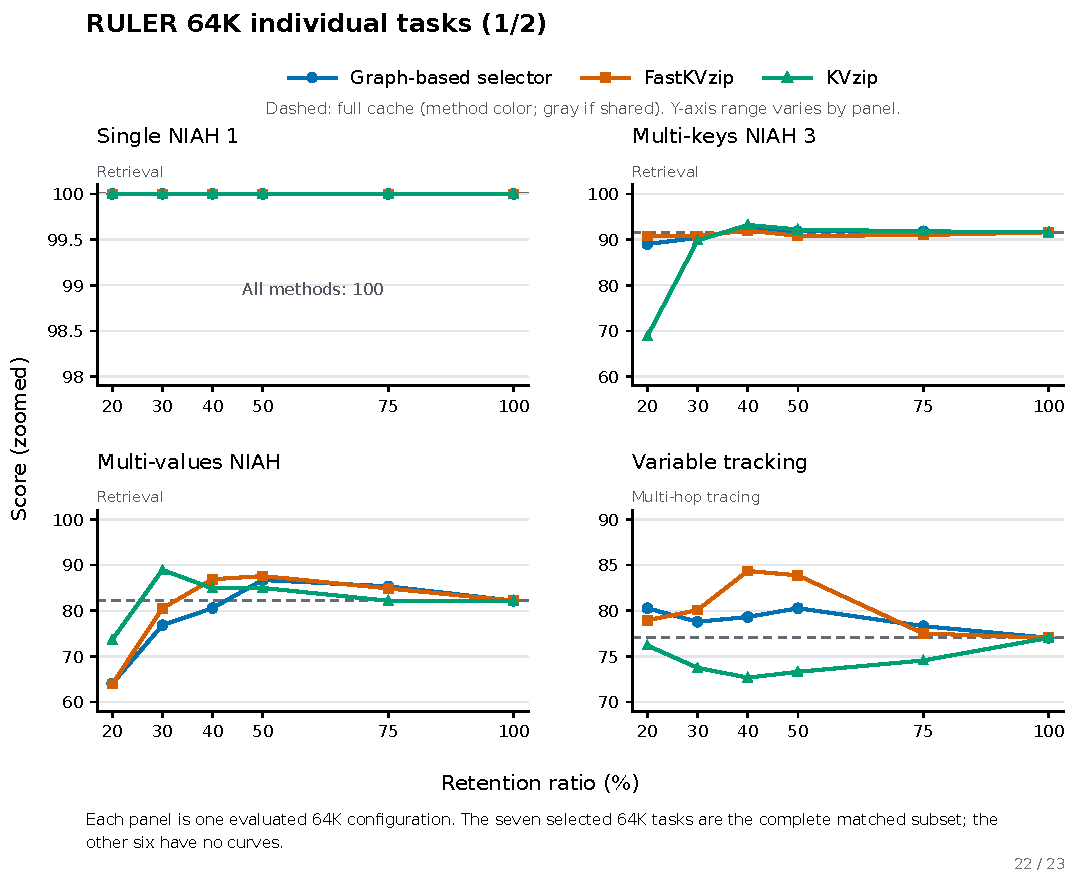
\includegraphics[width=\linewidth]{figures/retention-curves/22-ruler-64k-tasks-1.pdf}
\caption{RULER 64K individual tasks (1/2).}
\label{fig:retention-ruler-64k-tasks-1}
\end{figure}
\clearpage

\begin{figure}[!ht]
\centering
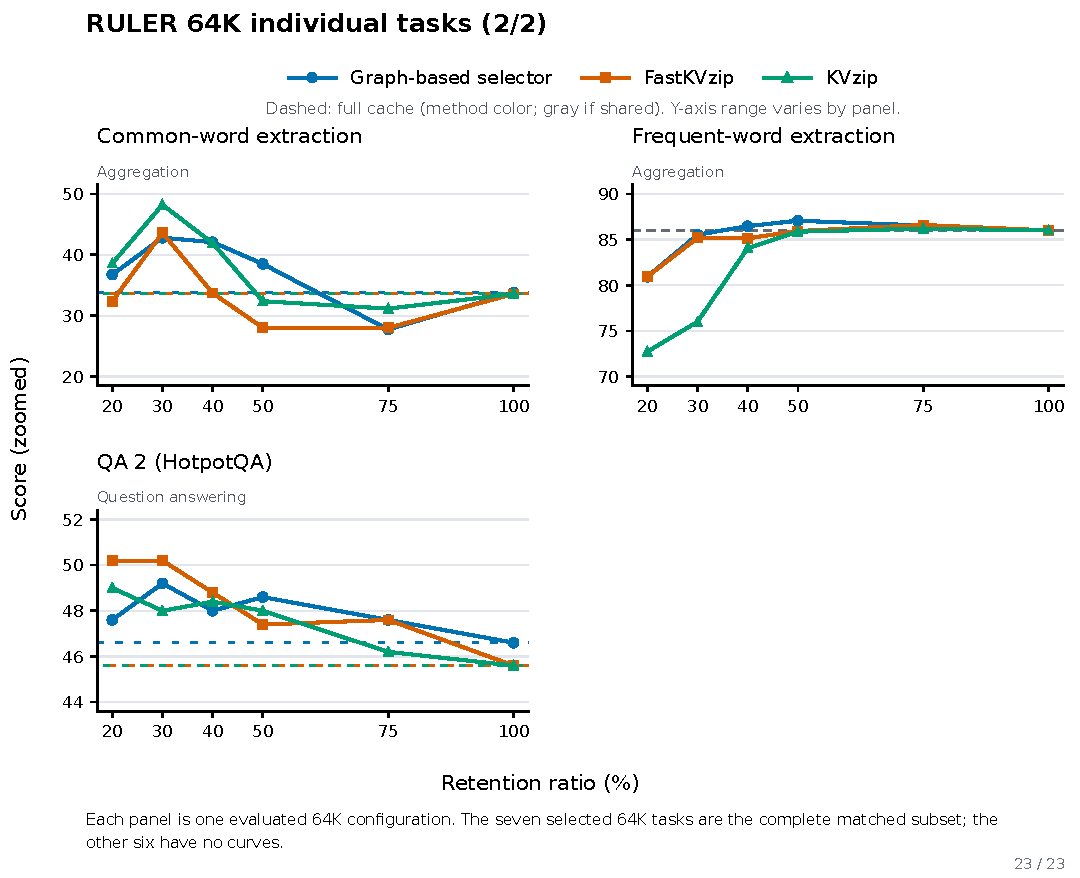
\includegraphics[width=\linewidth]{figures/retention-curves/23-ruler-64k-tasks-2.pdf}
\caption{RULER 64K individual tasks (2/2).}
\label{fig:retention-ruler-64k-tasks-2}
\end{figure}
\clearpage
